\documentclass[a1]{sciposter}

\usepackage{graphicx}
%\input amssym.def
%\input amssym
\usepackage{float}

\usepackage{lipsum}
\usepackage{epsfig}
\usepackage{amsmath}
\usepackage{amssymb}
\usepackage{multicol}
\usepackage{graphicx,url}
\usepackage[utf8]{inputenc}
%\usepackage{fancybullets}

\newtheorem{Def}{Definition}
%\noleftlogo
%\norightlogo
\nologos
\renewcommand{\titlesize}{\huge}
\renewcommand{\authorsize}{\large}
\renewcommand{\instsize}{\large}

\title{The optical properties of Hydrogen plasma described in the frame of the fully quantum method based on a cut-off Coulomb model potential}
\author{Nenad M.~Sakan$^{1}$*, Zoran J. Simi\'c$^{2}$, and Momchil Dechev$^{3}$}
\institute{\it $^{1}$ Institute of Physics, Belgrade University, Pregrevica 118, 11080 Zemun, Belgrade, Serbia\\
           $^{2}$ Astronomical Observatory, Volgina 7, 11060 Belgrade, Serbia\\
           $^{3}$ Institute of Astronomy and National Astronomical Observatory, Bulgarian Academy of Sciences, 72, Tsarigradsko chaussee Blvd. Sofia, Bulgaria}
\email{\bf nsakan@ipb.ac.rs}


\begin{document}

\maketitle

\conference{{\bf16tt ESPM - European Solar Physics Meeting, 6-10 September 2021, online}}

\begin{multicols}{3}
%%%%%%%%%%%%%%%%%%%%%%%%%%%%%%%%%%%%%%%%%%%%%%
%%%%%%%%%%%%%%%% ABSTRACT %%%%%%%%%%%%%%%%%%%%
%%%%%%%%%%%%%%%%%%%%%%%%%%%%%%%%%%%%%%%%%%%%%%

\begin{abstract}
The absorption coefficients of hydrogen plasma, calculated within the frame of cut-off Coulomb potential model, for the wide area of electron densities and temperatures observed within the solar atmosphere are presented here. The optical parameter of hydrogen plasma of mid and moderately high nonideality parameter could be described successfully, thus enabling the modeling of optical properties, especially the calculation of plasma opacity. The model was proven in both convergence towards normal condition, ideal plasma case, as well as with the help of analysis of the experimental data and further theoretical consideration. The model potential is solvable in entire space and within entire energy spectrum, thus the yielded wave function solutions are a combination of a special functions. The special form of the cut-of Coulomb potential, possesses an unique feature that enables the precise, fully quantum method of calculation of inverse Brehmstrahlung effect. Although the presented method development is still a work in progress the possibility of unifying a mode for both transport and optical properties of plasma within same model is an attractive direction for it’s further development
\end{abstract}


%%%%%%%%%%%%%%%%%%%%%%%%%%%%%%%%%%%%%%%%%%%%%
%%%%%%%%%%%%%%% SECTIONS %%%%%%%%%%%%%%%%%%%%
%%%%%%%%%%%%%%%%%%%%%%%%%%%%%%%%%%%%%%%%%%%%%%

\section{Introduction}

%%%%%%%%%%%%%%%%%%%%%%
% RAZMISLI KAKO DA IZMENIM OVO DO
%%%%%%%%%%%%%%%%%%%%%%

In the theoretical models of Solar plasma a problems of plasma opacity, energy transport as well as radiative transfer under moderate and strong non-ideality are of strong interest, for the deeper analysis of the subject reffere to \cite{for99, rog98, mih11, mih13}. The strong coupling and density effects in plasma radiation were the subject of numerous experimental and theoretical studies in the last decades. The presented quantum way of describing atomic photo-absorption processes in dense strongly ionized hydrogen plasma is based on the approximation of the cut-off Coulomb potential. By now this approximation has been used in order to describe transport properties of dense plasma (see e.g. \cite{for99, mih89, ign17}), but it was clear that it could be applied to some absorption processes in non-ideal plasmas too \cite{mih11,mih11c,mih15a,sak05}. More detailed explanation could be find in \cite{Sakan_atoms_2018}. 

%%%%%%%%%%%%%%%%%%%%%%
% DO OVDE
%%%%%%%%%%%%%%%%%%%%%%

\section{Theory}

\subsection{The approximation of the cut-off Coulomb potential}

Many body processes could be described by the use of transformation to the corresponding single-particle processes in an adequately chosen model potential, for the detailed theory \cite{Sakan_atoms_2018} should be considered.

As an adequate model potential for hydrogen plasma of higher density, for instance reffere to \cite{mih89,mih11}, the screening cut-off Coulomb potential, that satisfies above conditions, and is used here is in form
%%%%%%%%%%%%%%%%%%%%%%%%%%%%%%%%%%%%%%%%%%%%%%%%%%%%%%%%%%%%%%%%%%%%
\begin{equation}
\label{eq:U0} U_{c}(r) = \left\{
\begin{array}{c c}
- \displaystyle \frac{e^2}{r} + \displaystyle \frac{e^2}{r_c},
\qquad            0 < r \le r_{c},
\\
\displaystyle 0 ,              \qquad      r_{c} < r < \infty,
\end{array}
\right.
\end{equation}
%%%%%%%%%%%%%%%%%%%%%%%%%%%%%%%%%%%%%%%%%%%%%%%%%%%%%%%%%%%%%%%%%%%%
{\noindent where the mean potential energy of an electron
in the considered hydrogen plasma $U_{c}= -e^{2}/r_{c}$ is used as a energy origin of the potential. Here $e$ is the modulus of the electron charge, $r$ - distance from the ion, and cut-off radius $r_{c}$ - the characteristic screening length of the considered plasma.}

{\noindent The cut-off radius $r_{c}$ can be determined, see details in \cite{mih09b}. The code that calculates the characteristic screening length of considered plasma uses $N_{e}$ and $T$, and is given at {\it https://github.com/nsakan972/ESPM-16.git}, it is open sourced and free for use.}

\subsection{The calculated quantities}

In accordance with previously mentioned theory the behavior of the dipole matrix element is investigated. It is given by  $\hat{D}(r;r_{c};n_i,l_i;n_f,l_f) = $ $<n_f,l_f| {\mathbf r} |n_i,l_i>$,
where $|n_i,l_i>$ and $|n_f,l_f>$ are initial and final state wave functions obtained within the model of cut-off Coulomb potential. So all the photon emission and absorption parameters are related with the dipole matrix element. A essential calculation for this is the solving of the radial part of  Schr{\" o}dinger equation, e.g. finding of energy level values as well as the radial parts of the wave functions. The radial part, $R_{n,l;r_c}(r)$ presented as $\chi (r) = r R(r)$ for the selected level $n=3$ and $l = 0$ could be seen on Figure \ref{fig::1}. Please note that in the strong local plasma field a wave functions differ significantly from Coulomb case and as such reflect on all parameters and further calculated values.


%  *********   Start Figure 1  ****************
\begin{figure}
\begin{center}
\includegraphics[angle=-90,width=\textwidth]{fig/psi_n_3_l_0.eps}
\label{fig::1}
\end{center}
\end{figure}

\begin{center}
{{\bf Figure 1.} The plasma influence onto the form of wave function. Please note that $\chi (r) = r R(r)$, where $R(r)$ is a radial part of wave function.}
\end{center}

%  *********   End Figure 1 ****************

%%%%%%%%%%%%%


For instance the total absorption cross section is proportional to the dipole matrix element

\begin{equation}
\label{eq::Presek_totalni_dipolni}
    \sigma _0 (\omega = \omega _{fi}) \sim
    \left| \hat{D}(r;r_{c};n_i,l_i;n_f,l_f) \right| ^2,
\end{equation}

{\noindent and so any change of the wave function reflects on both dipole matrix element as well as total cross section symmetrically.}

%\begin{equation}
%\label{eq::Presek_totalni_dipolni}
%\sigma _0 (\omega = \omega _{fi}) = \frac{1}{3} \frac{g_2}{g_1}
%\frac{\pi \omega _{fi}}{\varepsilon _0 \hbar c}
%\hat{D}(r;r_{c};n_i,l_i;n_f,l_f) ^2.
%\end{equation}

The test set of dipole matrix elements for the hydrogen atom in plasma calculated for the variety of cut-off radius, $r_{c}$, values is available at {\it https://github.com/nsakan972/ESPM-16.git}. 

%\vfill\null
%\columnbreak

\section{Conclusion}

The presented work is a continuation of the previously developed modeling with for the photoionization and inverse Brehmsthrallung proceses of hydrogen plasma, and the goal is to include bond-bond processes within same model. All of previously calculated data is also usable in modeling of Solar plasma processes. 

In order to model a behaviour of the plasma optical characteristics the used potential is a good approximation for the modeling of plasma interaction in a large area of densities and temperatures, details in  \cite{Sakan_atoms_2018}.  A strong plasma influence onto the optical parameters is observed where the plasma interaction energy is close to observed level energy value, e,g. when this level starts to appear, as illustrated in figure. The work on using a more complex potentials is going on. We have tested a numerical method of wave function solution, and as a first step the Ar atom  modeled is introduced, and initial values are in a expected range. As a second effect, a more detailed plasma-emitter interaction could be modeled. For both experimental praxis as well as Sun processes modeling an introduction of He atom and ion model is must, and as such could determine the further research.

\begin{thebibliography}{99}

\bibitem[1]{for99} Fortov, V.E., Iakubov, I.T.~The physics of non-ideal plasma; World Scientific,  1999.

\bibitem[2]{rog98} Rogers, F.J., Iglesias, C.A.~ Opacity of stellar matter. Space Sci. Rev. 1998, 85,~61--70.
 
\bibitem[3]{mih11} Mihajlov, A.A., Sakan, N.M., Sre{\'c}kovi{\'c}, V.A., {Vitel}, Y., Modeling of continuous 
  absorption of electromagnetic radiation in dense partially ionized plasmas. J. Phys. A 2011, 44,~095502.
  
\bibitem[4]{mih13} {Mihajlov}, A.A.; {Ignjatovi{\'c}}, L.M., {Sre{\'c}kovi{\'c}}, V.A.,
  {Dimitrijevi{\'c}}, M.S., {Metropoulos}, A., The non-symmetric ion-atom radiative processes in the stellar, atmospheres, Mon. Not. R. Astron. Soc. 2013, 431,~589--599.
 
\bibitem[5]{mih89} Mihajlov, A.A., Djordjević, D., Popović, M.M., Meyer, T., Luft, M., Kraeft, W.D., Determination of the Electrical Conductivity of a Plasma on the Basis
  of the Coulomb cut-off Potential Model., Contrib. Plasma Phys., 1989, 29, ~441--446.
  
\bibitem[6]{ign17} {Ignjatovi{\'c}}, L.M., {Sre{\'c}kovi{\'c}}, V.A., {Dimitrijevi{\'c}}, M.S., The Screening Characteristics of the Dense Astrophysical Plasmas: The
  Three-Component Systems., Atoms, 2017, 5,~42.

\bibitem[7]{mih11c} Mihajlov, A.A., {Sakan}, N.M., {Sre{\'c}kovi{\'c}}, V.A., {Vitel}, Y., Modeling of the Continuous Absorption of Electromagnetic Radiation in Dense Hydrogen Plasma., 
  Balt. Astron., 2011, 20,~604--608.
  
\bibitem[8]{mih15a} {Mihajlov}, A.A., {Sre{\'c}kovi{\'c}}, V.A., {Sakan}, N.M., Inverse Bremsstrahlung in Astrophysical Plasmas: The Absorption
  Coefficients and Gaunt Factors., J. Astrophys. Astron., 2015, 36,~635--642. 

\bibitem[9]{sak05} {Sakan}, N.M., {Sre{\'c}kovi{\'c}}, V.A., {Mihajlov}, A.A., The application of the cut-off Coulomb potential for the calculation
  of a continuous spectra of dense hydrogen plasma., Mem. S. A. I. Suppl., 2005, 7,~221--224.

\bibitem[10]{Sakan_atoms_2018} Sakan, Nenad M. and Srećković, Vladimir A. and Simić, Zoran J. and Dimitrijević, Milan S., 
The Application of the Cut-Off Coulomb Model Potential for the Calculation of Bound-Bound State Transitions, Atoms, 2018, 6, 1, 4

\bibitem[11]{mih09b} Mihajlov, A., Vitel, Y., Ignjatovi{\'c}, L.M., The new screening characteristics of strongly non-ideal and dusty
  plasmas. Part 3: Properties and applications., High Temp., 2009, 47,~147--157.
  
\bibitem[12]{vit04} Vitel, Y., Gavrilova, T., D'yachkov, L., Kurilenkov, Y.K., Spectra of dense pure hydrogen plasma in Balmer area., J. Quant. Spectrosc. Radiat. Transf.,
  2004, 83,~387--405.

%\bibitem[1]{.} S. Autler and C. H. Townes,Contrib. Plasma Phys. Phys. Rev. A 10, 489 (1982). - for articles
%\bibitem[2]{.} E. U. Shirley, {\it The Theory of Molecules}, p. 399, (The University Press, Cambridge, 1954). - for books
%\bibitem[3]{.} C. E. Moore, ``Selected Tables of Atomic Spectra", NSRDS-NBS3, Setion 5, National Bureau of Standards, Washington, DC 20025 (1975). - for reports.
%\bibitem[4]{.} http://www.spig2012.pmf.uns.ac.rs - for web pages
\end{thebibliography}

\end{multicols}

\end{document}
